\chapter{Time Travel Debugging}\label{chapter-15-time-travel-debugging}

\begin{quote}
\textit{Replaying, rewinding, and re-steering computation across worldlines.}
\end{quote}

Most debuggers lie to you.

They present a convenient fiction: a single, linear narrative of execution. When you pause a program, they show you a stack trace, a breakpoint, a snapshot of memory, and perhaps a log file. Even the advanced ``time-travel'' debuggers currently on the market are essentially elaborate VCRs—they record state mutations so you can scrub the playhead backward.

But they all share the same fatal flaw. They show you the corpse of the process, not the life of it. They show you *what* happened, but they are architecturally incapable of showing you *why* it happened, or more importantly, *what almost happened*.

They fail to answer the questions that actually matter to a distributed systems engineer:

\begin{quote}
\textbf{What other worlds were possible at tick $T$?}

\textbf{Why did the system collapse into THIS worldline and not the others?}

\textbf{What would have happened if the scheduler had made a different, equally legal choice?}
\end{quote}

Traditional debugging tools cannot answer these questions because traditional computation has no geometry. It has no topology. It has no notion of a ``space'' of alternatives.

WARP+DPO (WARP Graphs + Double Pushout rewriting) changes that. In a WARP graph universe, debugging is not a reactive hunt for bugs. It is geometric navigation through a manifold of possibilities.

Welcome to **Time Travel Debugging**—a machine that allows you to walk backward through Chronos (sequential time), step sideways across Kairos (opportunity and choice), and move diagonally into parallel histories.

This is not science fiction. This is the inevitable utility of exposing the structure of possibility.

Let's ride.

\begin{center}
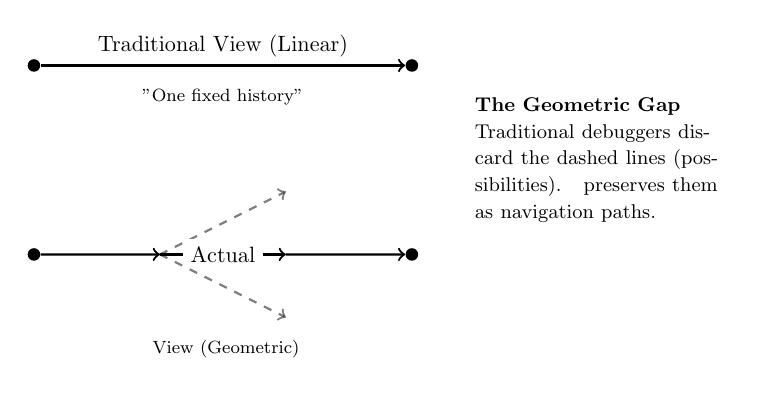
\begin{tikzpicture}[scale=0.8, transform shape]
    % Draw the "Lie" (Linear)
    \node (start1) at (0, 4) [circle, fill=black, inner sep=2pt] {};
    \node (end1) at (6, 4) [circle, fill=black, inner sep=2pt] {};
    \draw[->, thick] (start1) -- (end1) node[midway, above] {Traditional View (Linear)};
    \node at (3, 3.5) {\footnotesize "One fixed history"};

    % Draw the "Truth" (Branching)
    \node (start2) at (0, 1) [circle, fill=black, inner sep=2pt] {};
    \coordinate (mid) at (2, 1);
    \coordinate (branch1) at (4, 2);
    \coordinate (branch2) at (4, 1);
    \coordinate (branch3) at (4, 0);
    
    \draw[->, thick] (start2) -- (mid);
    \draw[->, thick, dashed, opacity=0.5] (mid) -- (branch1);
    \draw[->, thick] (mid) -- (branch2) node[midway, fill=white] {Actual};
    \draw[->, thick, dashed, opacity=0.5] (mid) -- (branch3);
    
    \node (end2) at (6, 1) [circle, fill=black, inner sep=2pt] {};
    \draw[->, thick] (branch2) -- (end2);
    
    \node at (3, -0.5) {\footnotesize \COMPUTER{} View (Geometric)};
    
    % Annotation
    \node[align=left, text width=4cm] at (9, 2.5) {\small \textbf{The Geometric Gap}\\Traditional debuggers discard the dashed lines (possibilities). \COMPUTER{} preserves them as navigation paths.};
\end{tikzpicture}
\end{center}

\section{Worldlines Store Their Own Geometry}

In a standard runtime, a history is a flat log:
\begin{verbatim}
State_0 -> State_1 -> State_2 -> ... -> State_N
\end{verbatim}

In \COMPUTER{}, a worldline is a rich geometric object. It doesn't just store the data that resulted from a computation; it stores the *context* of the transformation. 

At every tick of the clock, the system persists:
\begin{itemize}
    \item The **WARP** state (the graph).
    \item The **Bundle**: The set of all valid DPO rule matches that *could* have fired.
    \item The **Interference Pattern**: Which rules were mutually exclusive (critical pairs) and which were independent.
    \item The **Collapse**: The specific choice the scheduler made to resolve conflicts.
    \item The **Wormholes**: Legal connections to non-local states.
\end{itemize}

This means that every single tick of your program contains the formula:
$$ \text{Tick} = \text{History} + \text{Possibility} + \text{Geometry} $$

Time Travel Debugging is simply the act of replaying this geometric sequence while retaining the freedom to explore the branches that were pruned. Because the system is deterministic and the rules are structural, you can walk in any direction—even directions that ``didn't happen.''

\section{Rewinding Chronos}

Let's clarify the difference between ``undoing'' and ``rewinding.''

Traditional debugging implements time travel via brute force: it records the state of memory at interval $X$, and then stores differential snapshots. To go back, it reloads the snapshot and replays the mutations. It is shallow, brittle, and blind to the structure of the code.

\COMPUTER{} debuggers rewind Chronos by inverting the DPO rule.

Because every state transition is a graph rewrite rule $L \to R$ (Left-hand side to Right-hand side), and because we track the provenance of every node and edge, we can mathematically derive $R \to L$. We step backward through the applied rules, effectively running the physics of the universe in reverse.

This allows us to:
\begin{itemize}
    \item Reconstruct the prior WARP graph universe with perfect fidelity.
    \item Restore the ``bundle'' of potentiality that existed at that moment.
    \item Reveal the alternatives that were available *before* the choice was made.
\end{itemize}

This is fully reversible not because we have infinite storage, but because provenance is baked into the WARP graph. Time travel here is not state replay; it is **structural reconstruction**.

\section{Sidestepping Into the Time Cube}

This is where the paradigm shifts. Once you have rewound Chronos to a specific tick, you are not limited to looking at what *did* happen. You can look sideways.

We call this ``Sidestepping into the Time Cube.'' Imagine time (Chronos) as the Z-axis. The X and Y axes represent the space of valid transformations—the **Kairos**.

\begin{center}
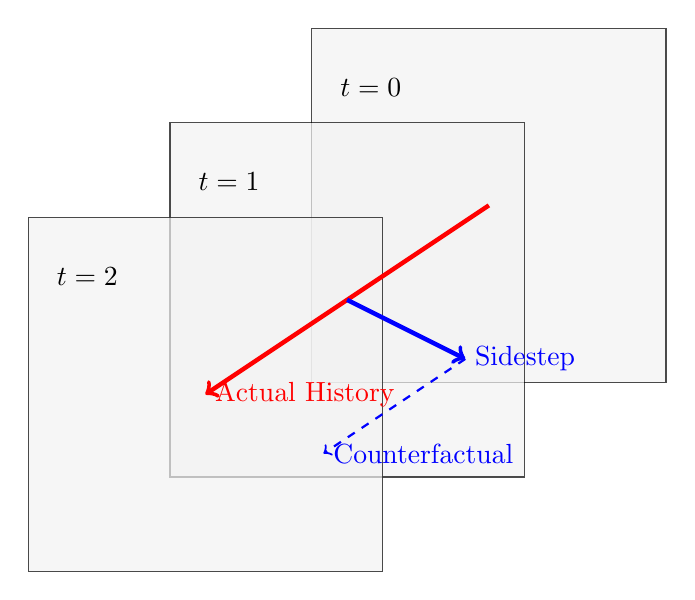
\begin{tikzpicture}[z={(-0.6cm,-0.4cm)}, x={(1cm,0cm)}, y={(0cm,1cm)}, scale=1.5]
    % Plane at t=0
    \draw[fill=gray!10, opacity=0.7] (0,0,0) -- (3,0,0) -- (3,3,0) -- (0,3,0) -- cycle;
    \node at (0.5, 2.5, 0) {$t=0$};
    
    % Plane at t=1
    \draw[fill=gray!10, opacity=0.7] (0,0,2) -- (3,0,2) -- (3,3,2) -- (0,3,2) -- cycle;
    \node at (0.5, 2.5, 2) {$t=1$};
    
    % Plane at t=2
    \draw[fill=gray!10, opacity=0.7] (0,0,4) -- (3,0,4) -- (3,3,4) -- (0,3,4) -- cycle;
    \node at (0.5, 2.5, 4) {$t=2$};

    % The Actual Path (Chronos)
    \draw[ultra thick, red, ->] (1.5, 1.5, 0) -- (1.5, 1.5, 2) -- (1.5, 1.5, 4);
    \node[red, right] at (1.5, 1.5, 4) {Actual History};

    % The Sidestep (Kairos)
    \draw[ultra thick, blue, ->] (1.5, 1.5, 2) -- (2.5, 1.0, 2);
    \node[blue, right] at (2.5, 1.0, 2) {Sidestep};
    
    % The Counterfactual
    \draw[thick, blue, dashed, ->] (2.5, 1.0, 2) -- (2.5, 1.0, 4);
    \node[blue, right] at (2.5, 1.0, 4) {Counterfactual};

\end{tikzpicture}
\end{center}

At any specific tick, you can pause and inspect the **Bundle**. This view reveals:
\begin{itemize}
    \item \textbf{Legal Alternatives:} What other rewrite rules matched the graph state?
    \item \textbf{Open Wormholes:} What remote interactions were possible?
    \item \textbf{Invariant Constraints:} Why did the system prune specific branches?
\end{itemize}

This is the moment traditional debuggers cannot show you: the adjacent futures. In the WARP worldview, debugging implies stepping sideways to inspect the ``road not taken.'' You aren't debugging the code; you are debugging the *physics* of your computational universe to understand why the probability collapsed the way it did.

\section{Forward Into Counterfactual Worldlines}

Now comes the fun part. Once you have rewound to $t=100$, and sidestepped to select an alternative rule that *could* have fired, you can press ``Play.''

This creates a **Counterfactual Worldline**.

\begin{quote}
A ``what-if'' version of history that respects all system invariants, all legal rewrites, and the same DPO ruleset, but originates from a different choice.
\end{quote}

It is crucial to understand that you are not guessing. You are not running a stochastic simulation or fuzzing the inputs. You are following the **real, legal future** that the universe *would have had* if the scheduler had picked option B instead of option A.

This allows for safe, deterministic counterfactual execution. No approximation. No branching explosion. Just geometry.

\section{Multi-World Time Travel (MWTT)}

The real power of \COMPUTER{} emerges when you combine these movements into a unified workflow. MWTT is a machine that allows you to:
\begin{enumerate}
    \item Rewind Chronos to a divergence point.
    \item Sidestep into Kairos to select a different branch.
    \item Follow the new worldline forward.
    \item Compare the two timelines simultaneously.
\end{enumerate}

This enables a new class of engineering analysis:
\begin{itemize}
    \item \textbf{Divergence Analysis:} How quickly do two similar states drift apart?
    \item \textbf{Brittleness Detection:} Does a minor change in scheduling order cause a catastrophic failure in the logic?
    \item \textbf{Curvature Traps:} Are there states that act as ``black holes,'' sucking all possible futures into a deadlock?
    \item \textbf{Geodesic Finding:} What was the shortest path to the error?
\end{itemize}

This is multi-world debugging, but it remains deterministic. Each branch is just a different valid collapse of the wave function. Each worldline is a distinct path through the Rulial manifold.

\section{Debugging By Comparison: Worldline Diffing}

We are all familiar with `git diff`. It shows the textual difference between two static files. But how do you diff a *process*?

Time Travel Debugging enables **Worldline Diffing**. Imagine a tool that overlays the ``Actual Worldline'' (where the bug occurred) with an ``Ideal Worldline'' (a counterfactual where the system behaved correctly) or a ``Hypothetical Worldline'' (where a race condition resolved differently).

Worldline diffs reveal the topology of divergence:
\begin{itemize}
    \item **Where** the universes split (the exact tick).
    \item **Why** they split (the rule conflict).
    \item **The Rulial Distance:** A metric of how structurally different the two universes have become.
    \item **Invariant Pressure:** Which constraints forced the collapse in one direction versus the other.
\end{itemize}

This is the computational equivalent of a semantic diff for physics.

\section{Practical Examples}

How does this look in practice?

\textbf{Debugging a Game Engine (Physics glitch):}
The player fell through the floor.
\begin{itemize}
    \item Rewind to the tick before the collision check.
    \item Sidestep to view the bundle. You see the collision rule *matched*, but was preempted by a ``network correction'' rule.
    \item Force the collision rule. Watch the counterfactual worldline where the player stands firmly on the ground.
    \item Diagnosis: Network latency correction has higher priority than local physics.
\end{itemize}

\textbf{Debugging a Compiler (Optimization error):}
The generated IR is invalid.
\begin{itemize}
    \item Rewind to the optimization pass.
    \item Trace the alternative rewrites. You see a ``Loop Unroll'' and a ``Dead Code Elimination'' competing.
    \item Follow the path where ``Dead Code'' fires first. The IR remains valid.
    \item Diagnosis: The optimization pass order is non-confluent.
\end{itemize}

\textbf{Debugging a Distributed System (Race condition):}
A database transaction was lost.
\begin{itemize}
    \item Rewind to the message arrival.
    \item Sidestep into the simultaneous legal transitions.
    \item Explore the consistent outcomes versus the actual inconsistent one.
    \item Diagnosis: The consensus algorithm allowed a commit before the lock was fully propagated.
\end{itemize}

This is not theory. This is a machine. A real-world tool made possible by the rigor of WARP+DPO.

\begin{nerdbox}
\textbf{MWTT $\approx$ Traversal of the Rulial Neighborhood Graph}

For those formally inclined, Multi-World Time Travel is essentially the interactive traversal of local Rulial surfaces.

\begin{itemize}
    \item \textbf{Peak-Join Diagrams:} When we ``sidestep,'' we are inspecting the Critical Pairs $(t_1 \leftarrow s \to t_2)$.
    \item \textbf{Confluence Analysis:} When we check if two worldlines converge, we are testing the Church-Rosser property for that local region.
    \item \textbf{Equivalence Classes:} ``Diffing'' worldlines is often a search for traces that are permutationally equivalent.
\end{itemize}

\COMPUTER{} simply expresses these abstract reduction strategies as geometric navigation tools, allowing engineers to intuitively surf the Rulial Neighborhood Graph without needing a PhD in category theory.
\end{nerdbox}

\section{Transition: From Debugging to Counterfactual Engines}

We have established that we can rewind Chronos, explore Kairos, follow alternative futures, and analyze the bundles of possibility.

If we can do this manually in a debugger, we can automate it.

We can build a machine that systematically explores these parallel universes for the purposes of search, optimization, verification, and adversarial analysis. We can turn the debugger into a generator.

That is the subject of Chapter 16.

Time to surf the multiverse.
